\documentclass[a4paper,12pt,spanish,notitlepage]{report}
\usepackage[spanish]{babel}
\usepackage{graphicx}
\usepackage[utf8]{inputenc}
\usepackage{color}
\usepackage{hyperref}
\usepackage{tikz}
\usepackage[all]{hypcap}
\usepackage[section]{placeins}
\usepackage{wrapfig}
\usepackage{float}
\usepackage[top=1.5in]{geometry}
\newcommand{\executeiffilenewer}[3]{%
\ifnum\pdfstrcmp{\pdffilemoddate{#1}}%
{\pdffilemoddate{#2}}>0%
{\immediate\write18{#3}}\fi%
}
\newcommand{\includesvg}[1]{%
\executeiffilenewer{#1.svg}{#1.pdf}%
{inkscape -z -D --file=#1.svg %
--export-pdf=#1.pdf --export-latex}%
\input{#1.pdf_tex}%
}
\renewcommand{\ttdefault}{lmtt}
\usetikzlibrary{calc,trees,positioning,arrows,chains,shapes.geometric,%
    decorations.pathreplacing,decorations.pathmorphing,shapes,%
    matrix,shapes.symbols}
\tikzset{
>=stealth',
  punktchain/.style={
    rectangle, 
    rounded corners, 
    % fill=black!10,
    draw=black, very thick,
    text width=10em, 
    minimum height=3em, 
    text centered, 
    on chain},
  line/.style={draw, thick, <-},
  element/.style={
    tape,
    top color=white,
    bottom color=blue!50!black!60!,
    minimum width=8em,
    draw=blue!40!black!90, very thick,
    text width=10em, 
    minimum height=3.5em, 
    text centered, 
    on chain},
  every join/.style={->, thick,shorten >=1pt},
  decoration={brace},
  tuborg/.style={decorate},
  tubnode/.style={midway, right=2pt},
}
\def\etc{\textsl{etc}}
\def\eg{\textsl{eg.}\ }
\def\etal{\textsl{et al.}}
\renewcommand\quote[1]{\lq\textsl{#1}\rq}
\newcommand\fr[2]{{\textstyle\frac{#1}{#2}}}
\def\name{\textsl{Ni intento Entertainment Kernel}}

\begin{document}
\title{
\centering{
\includegraphics[width=10cm]{NES_logo.png}}}
\author{Martín Villagra}
\maketitle
\vspace{1cm}
\centering{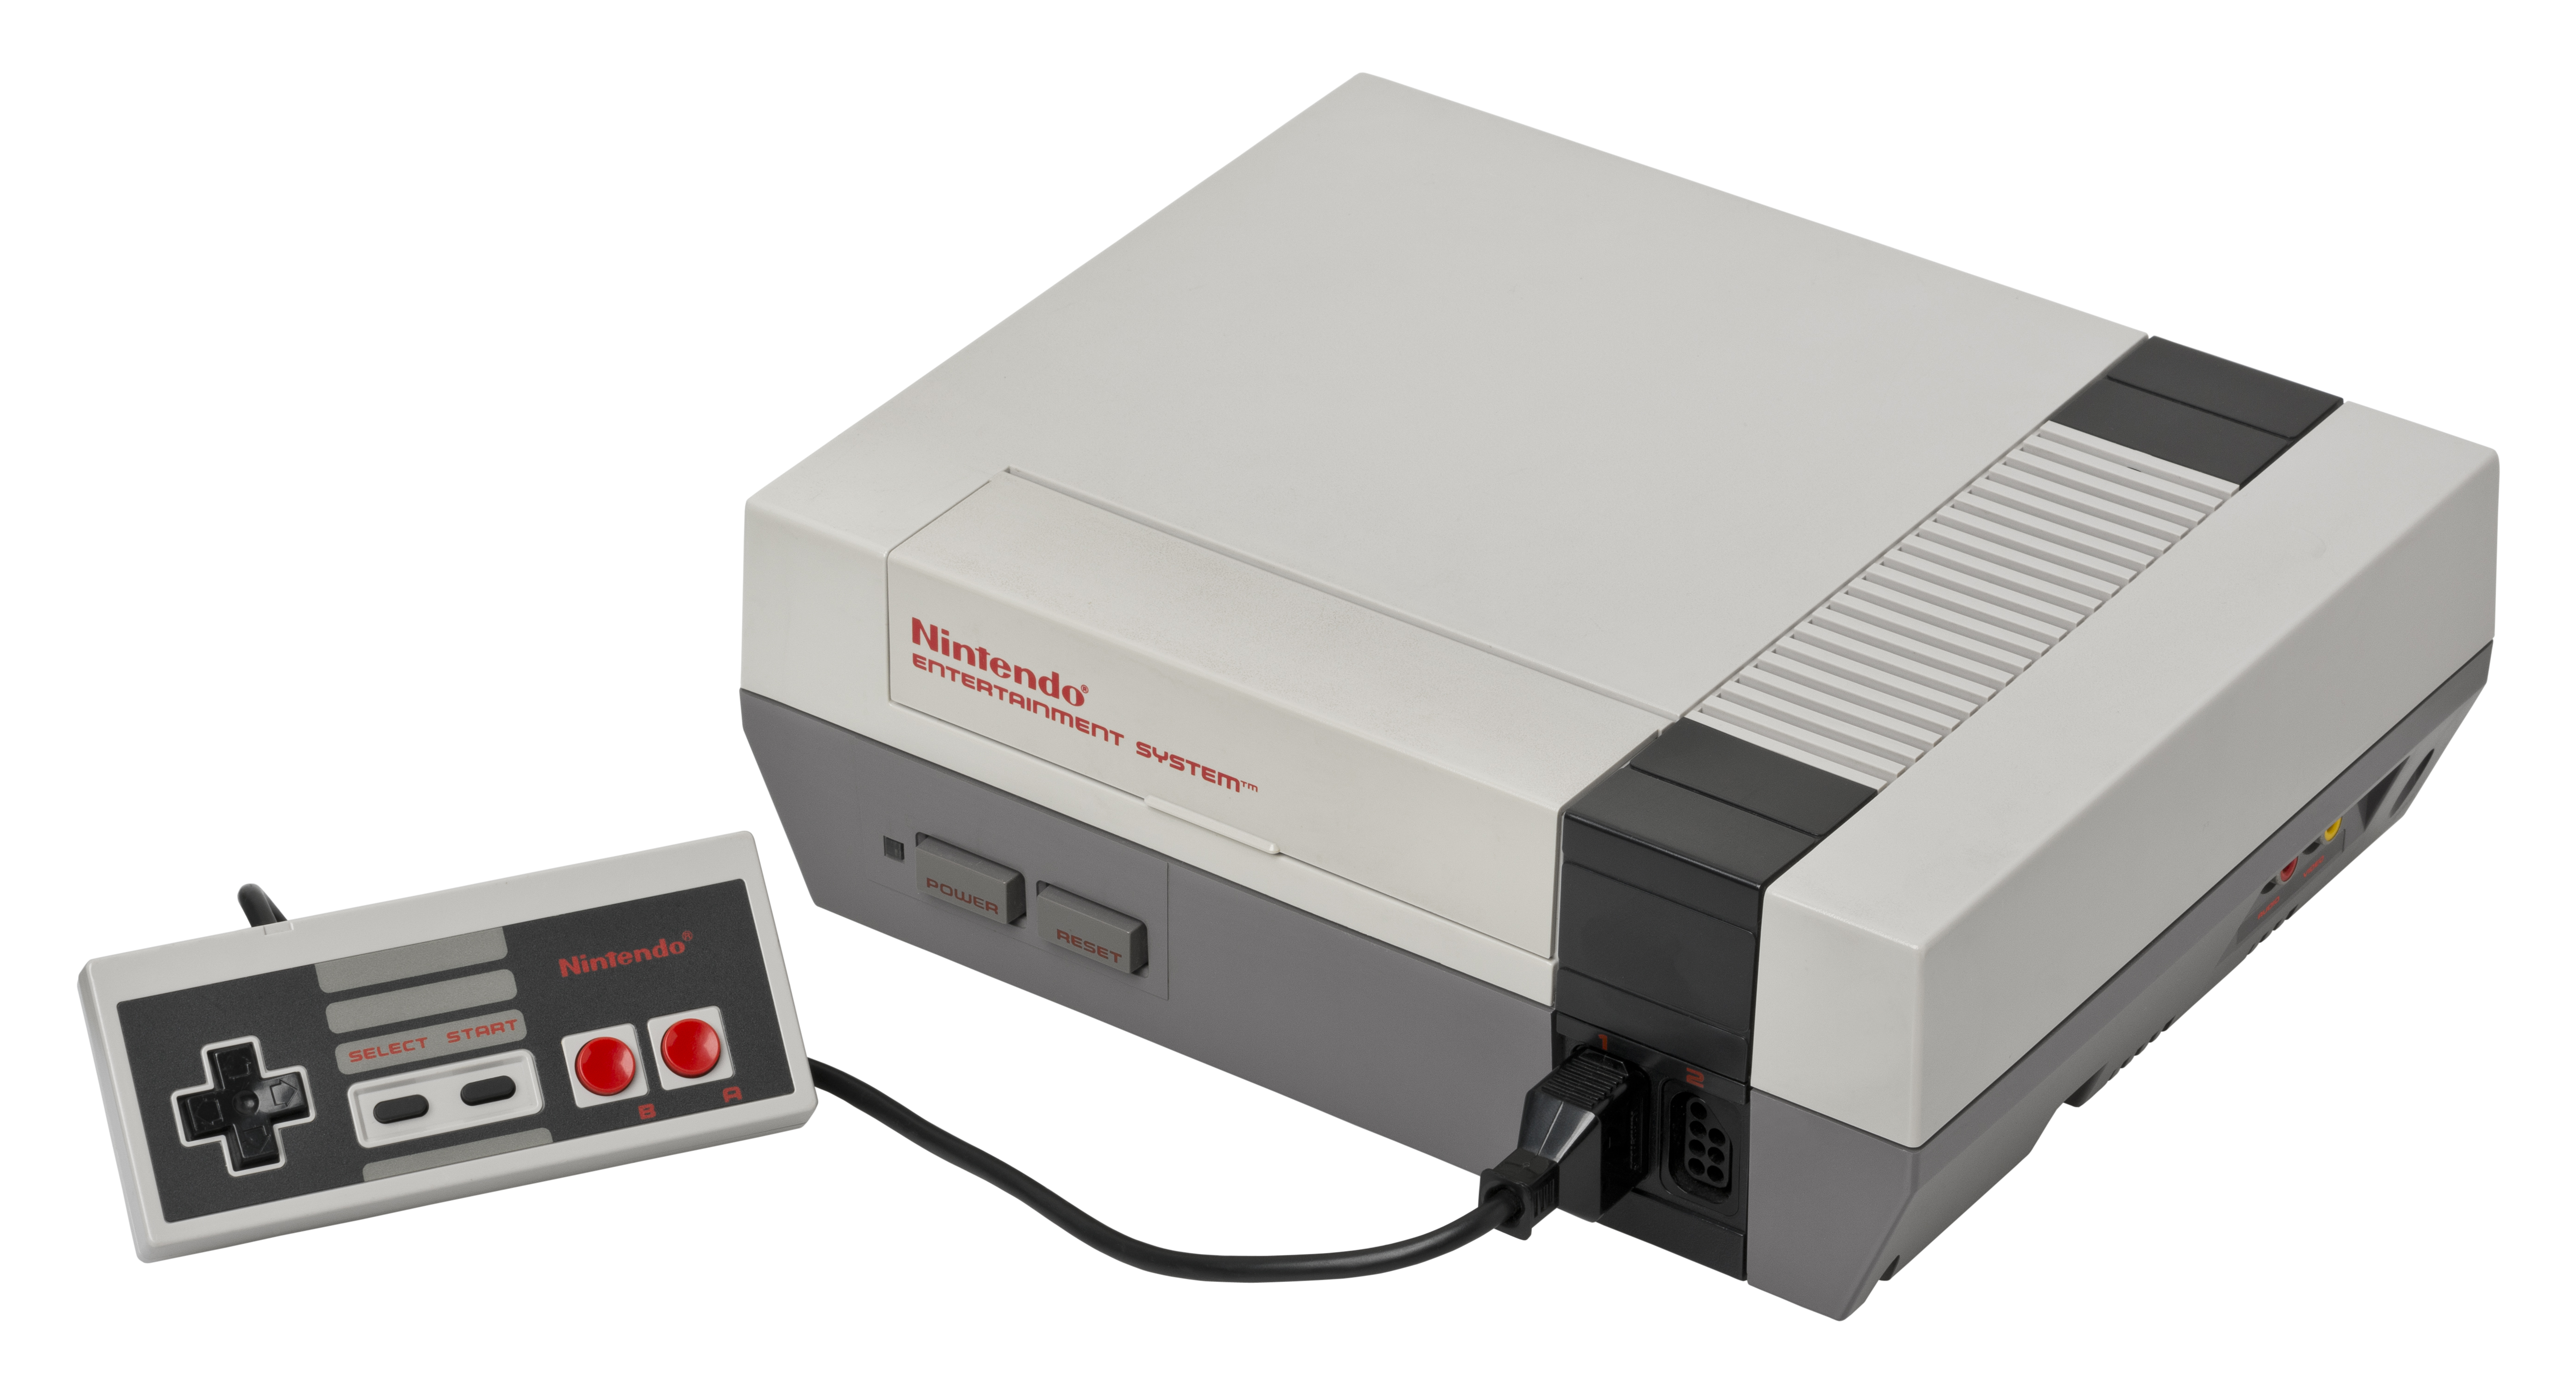
\includegraphics[width=15cm]{NES-Console-Set.jpg}}
\vspace{\fill}
\begin{abstract}\centering
El objetivo del trabajo es construir un emulador de la videoconsola Nintendo Entertaiment System(también conocida como Family) que se ejecute sin ningún sistema operativo de por medio.
\end{abstract}
\raggedright
%-----------------------------------------------------------
\tableofcontents
%-----------------------------------------------------------
\chapter{Introducción}
La consola NES\footnote{\url{http://en.wikipedia.org/wiki/Nintendo_Entertainment_System}}fue una de las consola más vendidas de todos los tiempos. En 2009, la misma fue nombrada la mejor consola de videojuegos de la historia por IGN\footnote{\url{http://uk.ign.com/top-25-consoles/1.html}}.
Gracias a su popularidad y simplicidad muchas personas se interesaron en el funcionamiento de la consola, dando lugar a una abundante documentación al respecto.

Fue por estas dos razones que se dicidió emular está consola en particular.

Por otro lado, se eligió realizar un kernel para no depender de ningún sistema operativo. Esto introduce la posibilidad de ejecutar el emulador en máquinas más restringidas, que obviamente resultarían de menor costo que una computadora o la consola original.

Debido a la gran extensión del trabajo, se decidió seguir la filosofía de no reinventar la rueda. El proyecto se construyó tomando como base otros kernels y emuladoras ya existentes.

\section{Estructuración}

En un principio dividimos en dos partes principales el projecto.

Una es el \textbf{emulador} propiamente dicho, es decir la que se encarga de hacer todo lo que hacía internamente la consola.

La otra parte es el \textbf{kernel} encargada de inicializar todo lo necesario para que el emulador funcione, así como proveerle funciones de bajo nivel tales como escribir en pantalla o reservar memoria. Al no tener un sistema operativo detrás, funciones como malloc y free que cualquier programador de C supone siempre presentes deben ser implementadas por el kernel.

\def\kernel{\textbf{kernel} }
\def\SO{\textbf{kernel} }
\chapter{El Kernel}

Un \kernel (de la raíz germánica Kern, núcleo, hueso) se define como la parte que se ejecuta en modo privilegiado (conocido también como modo núcleo), es decir con acceso irrestricto a todo el hardware del sistema. Es el principal responsable de facilitar a los distintos programas acceso seguro al hardware de la computadora y de  gestionar recursos.

En su más simple escencia es simplemente un código ejecutable, el cual es generado con un compilador como cualquier otro. La diferencia es que no tiene dependencias con librerías del sistema, tales como stdio.h o stdlib.h.

\section{Carácteristicas}
Empecemos por decir que lo que aquí se presenta está muy lejos de un sistema operativo completo. Se priorizó la simplicidad recortando todo lo que estaba de más, reduciendo al mínimo las capacidades del sistema. Por ejemplo la mayoría de los sistemas operativos pueden leer un programa y ejecutarlo. Nuestro querido kernel carece de esa posibilidad. A continuación se enumeran las carácteristicas principales del sistema.

\begin{itemize}
\item Dentro de la familia de arquitecturas x86\footnote{\url{http://en.wikipedia.org/wiki/X86}} se eligió i686\footnote{\url{http://en.wikipedia.org/wiki/P6_(microarchitecture)}}. Se prefirió esta por sobre x86\_64\footnote{\url{http://en.wikipedia.org/wiki/X86-64}} ya que tiene esta última no es soportada nativamente por GRUB(ver sección ~\ref{sec:booteo}). Respecto al formato de los ejecutables se eligió el que implementan los sistemas Unix\footnote{\url{http://en.wikipedia.org/wiki/Unix}}(como Linux\footnote{\url{http://en.wikipedia.org/wiki/Linux}}), el ELF \footnote{\url{http://en.wikipedia.org/wiki/Executable_and_Linkable_Format}}.
\item Es un kernel \underline{monolítico}, esto significa que todos los drivers y los servicios necesarios para el funcionamiento completo del sistema están incluídos en dentro del mismo kernel. Sistemas operativos como Linux no siguen esta filosofía, ya que implicaría cargar todos los drivers al incio del sistema, el cual tiene un costo de memoria muy alto. Esto no representa un problema para nosotros puesto que la cantidad de drivers y servicios ofrecidos por el kernel es muy reducida.
\item \underline{Monotarea}: Solo puede realizar una tarea a la vez, en nuestro caso el emulador. Para simplificar aún más incluso, el emulador es verdaderamente la \emph{única} tarea que el kernel puede ejecutar. Podría verse al emulador como un solo programa standalone, que no necesita ningún sistema operativo para ejecutarse.
\item Sin \underline{memoria virtual}: En un sistema operativo clásico cada proceso tiene sus propio mapa de direcciones virtuales. A medida que el proceso va solicitando más memoria se busca espacio en la memoria física y luego se le asigna la encontrada a una dirección virtual, la cual es usable por el proceso. Este sistema tiene ventajas tales como la posibilidad de restringir la memoria accesible por un proceso. Es destacable que la memoria física no tiene porque restringirse solo a la RAM\footnote{Random Access Memory}, puede apuntar incluso a una posición en el disco duro. Optamos por no incluir esta opción, para simplificar el sistema. Esto significa que los punteros contienen la dirección de memoria física y que es posible acceder y leer la memoria usada por otros procesos libremente.
\item Sin \underline{userspace}: Normalemente un sistema operativo puede dividirse en tres capas de abstracción diferentes, el hardware, el kernel y finalmente el userspace, que es donde se ejecutan las aplicaciones como Chromium, Notepad, \etc.
\end{itemize}
\begin{figure}[h]
\centering
\def\svgwidth{5cm}
\input{Kernel_Layout.pdf_tex}
\caption{Layout estándar de un kernel.}
\end{figure}
\FloatBarrier
En nuestro caso no tenemos userspace: el emulador, nuestro único programa a ejecutar, está embebido en el mismo kernel. Esto simplifica enormemente el diseño del kernel.

\section{Funciones}
Antes de hacer el kernel, hay que tener muy en claro que es exactamente lo que tiene que hacer. Surge la pregunta entonces ¿Qué necesita como mínimo nuestro emulador? Se muestra, en orden de importancia:
\begin{itemize}
\item Iniciar el sistema y ejecutar el emulador. Ver sección ~\ref{sec:booteo}.
\item Modificar libremente pixeles de la pantalla
\item Detectar pulsaciones del teclado
\item Poder reservar memoria dinámica *explicar que es*
\item Cargar de alguna forma los juegos
\item Ejecutar sonido
\item Escribir en algún medio persistente el estado actual del juego(Guardar la partida)
\end{itemize}
Pues bien, el kernel tiene que ser capaz de proveer funciones que faciliten cada una de estas tareas. En las siguientes secciones se detallaran cada una de ellas.

\section{Booteo}\label{sec:booteo}
*explicar que es un bootloader y la bios muy brevemente*
Para evitar tener que lidiar con la BIOS y otras interfaces de bajo nivel, se eligió utilizar un bootloader ya existente y ampliamente usado: GRUB. *poner que carajos es GRUB*. En particular existe un standard llamado Multiboot\footnote{\url{http://en.wikipedia.org/wiki/Multiboot_Specification}} que especifica como estructurar un kernel para que el mismo pueda ser cargado por GRUB(o por cualquier otro bootloader que implemente Multiboot). En particular se debe elaborar un header al inicio del kernel. En esta cabecera se determina por ejemplo que modo se prefiere(texto o consola) y que función va a ser la primera en ser llamada. A su vez GRUB se comunica con la BIOS entre otras cosas y recolecta información de la máquina que luego es recibida convenientemente por nuestro kernel. De esta forma al encender la máquina se iniciará GRUB, el mismo va a poder detectar nuestro kernel y lo va a ejecutar.

\subsection[boot.s]{boot.s\protect\footnotemark{}\protect\footnotetext{Ubicado en kernel/arch/x86/generic/init/boot.s}}
El problema es que al momento en que GRUB ejecuta el kernel el stack pointer no está inicializado por lo que no es posible que la función inicial sea en C. Debemos comenzar en assembler, inicializar el stack pointer y ahí si pasar a C. Esta es la razón de la existencia del archivo boot.s, que contiene el comienzo de nuestro kernel. Allí se incluye el header de Multiboot, el espacio para el stack y una función, la primera en ser llamada al iniciar el sistema, que inicializa el stack pointer y llama a nuestra función kernel\_entry\footnote{Ubicado en kernel/arch/x86/generic/init/kernel\_entry.c}(ya en C) que continua con la inicialización del sistema.

\chapter{Emulador}
\begin{wrapfigure}{r}{0.6\textwidth}\caption{Placa madre de la consola\label{fig:hardware}}
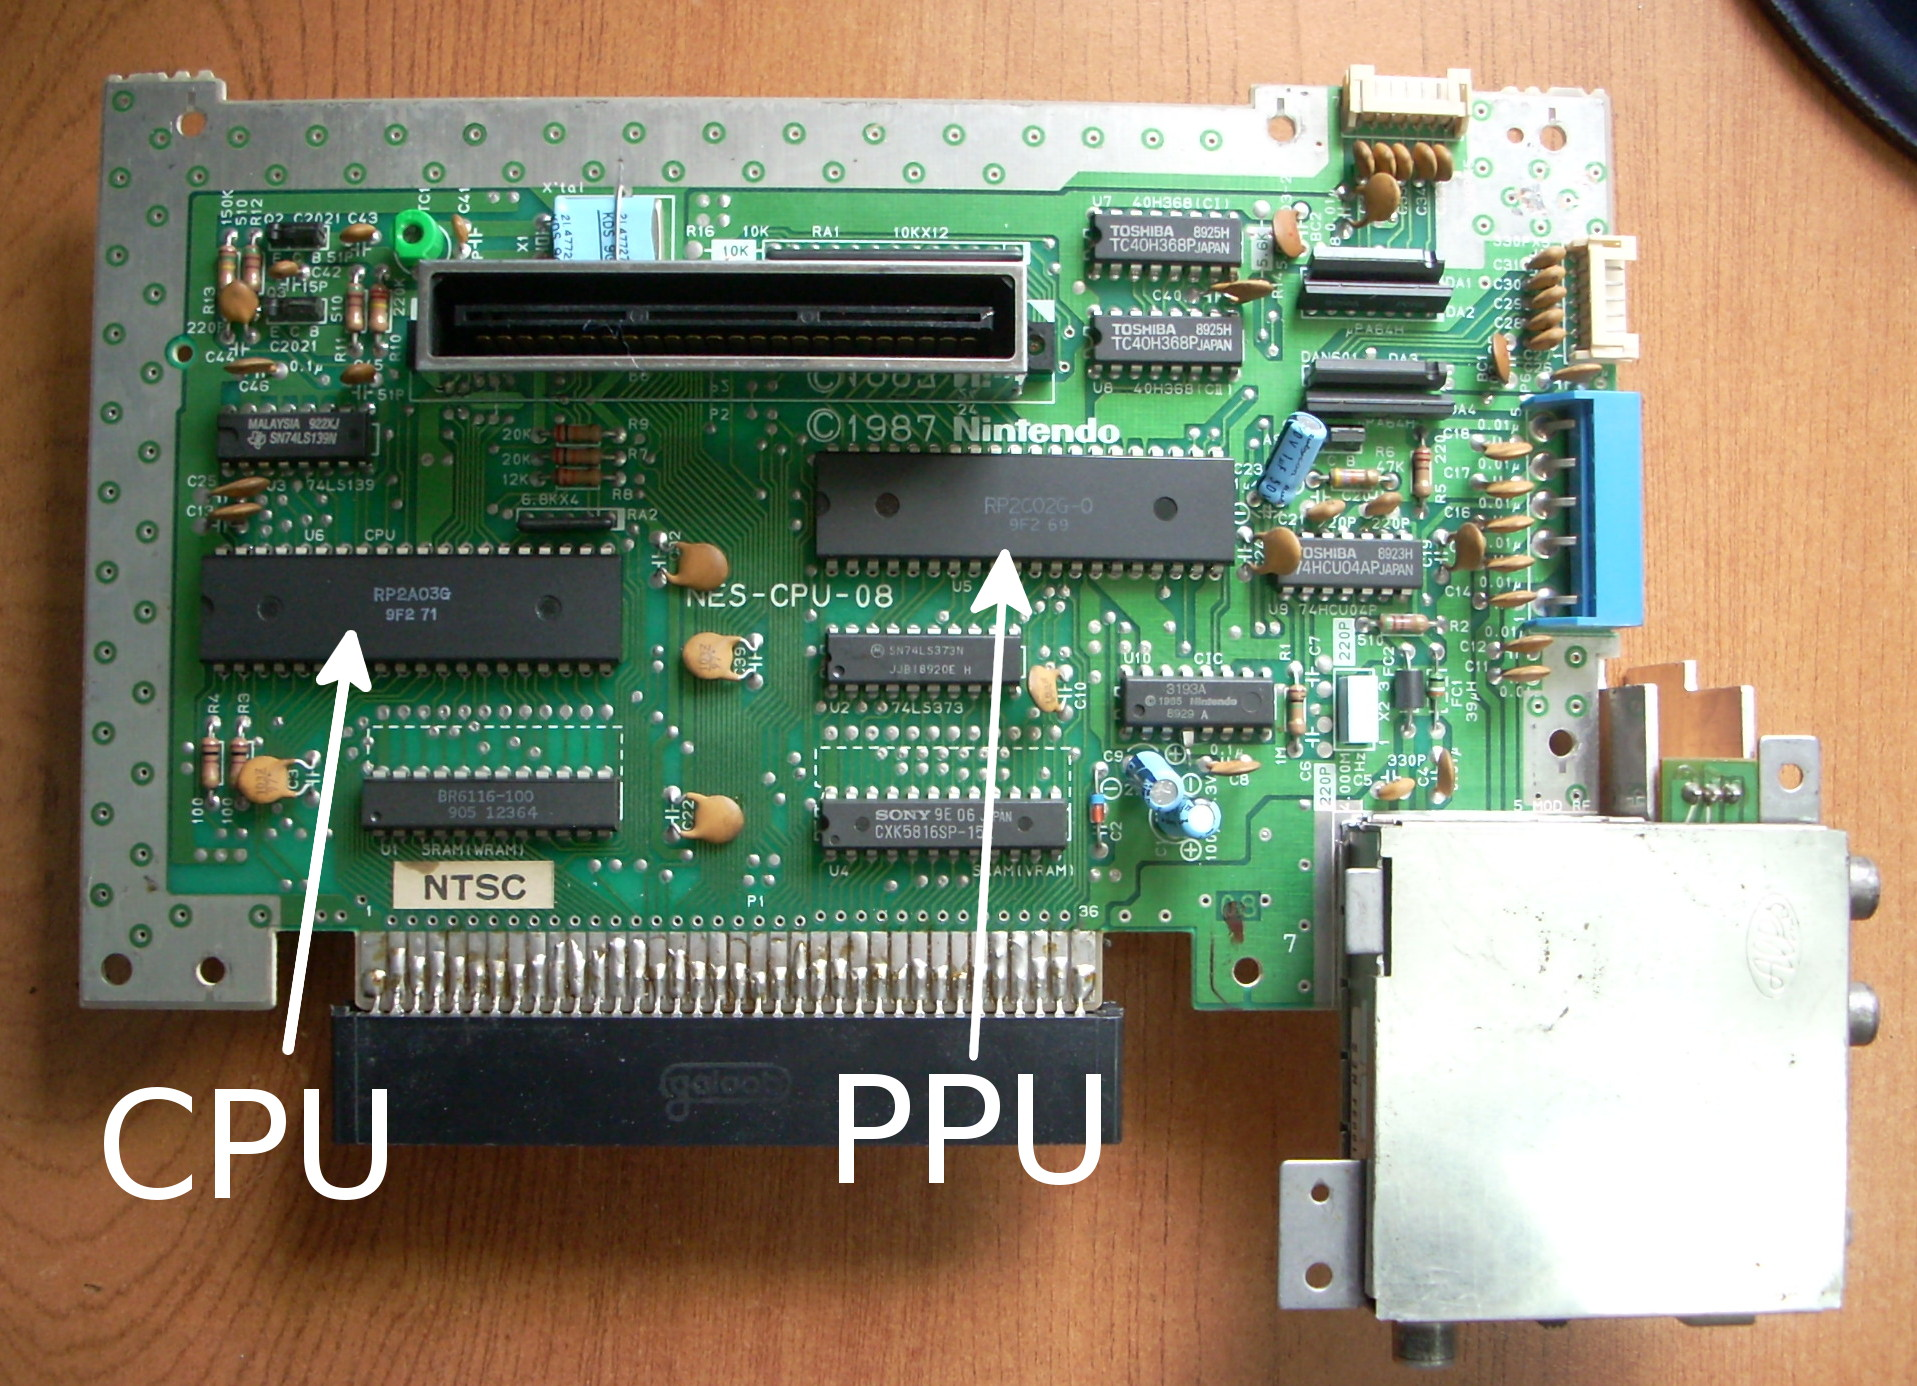
\includegraphics[width=0.6\textwidth]{hardware.jpg}
\end{wrapfigure}
La intención de que la consola sea más barata que la competencia de la época llevaron a que Nintento se decida a usar una Unidad de Procesamiento Central (CPU) desactualizada. Si bien un procesador de 16-bit hubiera sido lo óptimo, para mantener los precios bajos se decidieron a usar una variante del procesador 6502 de 8 bits, desarrolado por MOS techonology en 1975. El chip bastaría para ejecutar los programas, pero sería incapaz de generar los gráficos requeridos por lo que la compañía dicidió usar un segundo chip como una unidad totalmente dedicada al procesamiento de imagenes (Picture Processing Unit, PPU), responsable de calcular y mostrar los gráficos.



Ambos chips tienen su propia memoria interna, en forma de RAM. Los juegos son usualmente guardados en chips ROM\footnote{Read Only Memory} dentro del cartucho, el cual es accedido por la CPU cuando los mismos son insertados en el sistema.
La NES usa memory mapped I/O\footnote{Input/Output} para permitir al procesador comunicarse con sus otros componentes: la PPU y los dispositivos de entrada. La memory mapped I/O es una técnica donde la información puede ser transferida a un dispositivo mediante la escritura en una dirección espécifica en la memoria.


\section{CPU Memory Map}
\begin{figure}[H]\caption{Buses de la consola\label{fig:bus}}
\centering{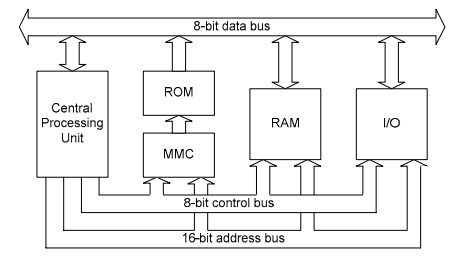
\includegraphics[width=0.8\textwidth]{bus.png}}
\end{figure}
La memoria está dividida en tres partes, la ROM dentro de los cartuchos, la RAM de la CPU y los registros I/O. El bus de direcciones es usado para establecer la dirección deseada. El bus de control es usado para informar a los componentes si el pedido es de lectura o escritura. El bus de datos es usado para leer o escribir el byte a la dirección elegida. Notemos que la ROM es de solo lectura y es accedida via el MMC, para permitir el cambio de bancos (explicado más abajo). Los registros I/O son usados para comunicarse con los otros componentes del sistema: la PPU y los dispositivos de entrada.

El chip 2A03 presente en la consola tiene un bus de direcciones de 16-bit y como tal puede soportar 64 KB de memoria en el rango \$0000-\$FFFF. La figura ~\ref{fig:memorymap} muestra el mapeo de memoria usado por la NES. El lado izquierdo es una versión simplificada mostrando las secciones más importantes, mientras que el lado derecho detalla cada sección.
\begin{figure}[H]\caption{Mapeo de la memoria\label{fig:memorymap}}
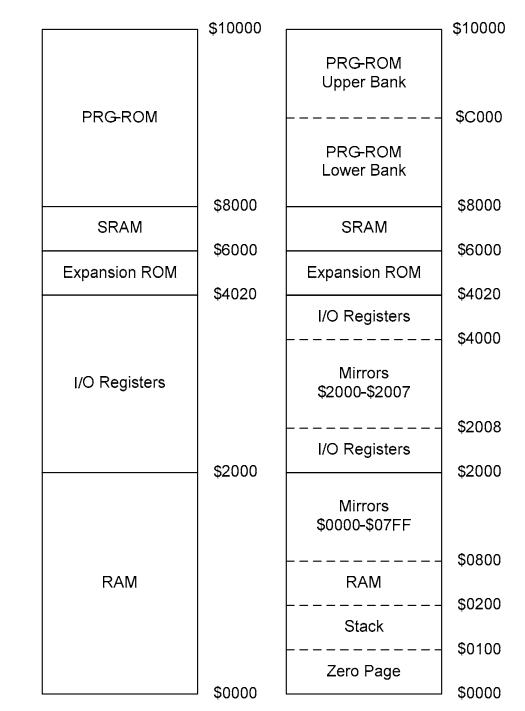
\includegraphics[width=0.8\textwidth]{memorymap.png}
\end{figure}


Zero Page se refiere a las direcciones en el rango \$0000-\$00FF, la primera página en memoria. La misma es usada por ciertos modos de acceso para lograr una ejecución más veloz. Las direcciones  \$0000-\$07FF están espejadas tres veces en \$0800-\$1FFF. Esto significa que por ejemplo, cualquier información escrita en \$0000 también se escribirá en \$0800, \$1000 y \$1800. Las direcciones \$2000-\$2007 están espejadas cada 8 bytes en la región \$2008-\$3FFF y los restantes registros siguen este espejado. SRAM (o WRAM) es la RAM de guardado, espacio usado para guardar las partidas.

A partir de \$8000 se encuentra la PRG-ROM\footnote{Program ROM} del cartucho. Juegos con solo un banco de 16 KB de PRG-ROM se cargaran tanto en \$8000 como en \$C000. Juegos con dos bancos de 16 KB de PRG-ROM, cargaran uno en \$8000 y otro en \$C000. Juegos con más de dos bancos usan mamory mappers para determinar que banco cargar en memoria. El memory mapper vigila las escrituras a una dirección específica (o rango de direcciones) y cuando esa dirección es escrita, realiza un cambio de bancos\footnote{Hace que la memoria mapee hacia un banco distinto al que se estaba usando}. Los detalles varían entre diferentes memory mappers. 

\section{Registros}
El 6502 tiene menos registros que procesadores similares. Existen tres registros especiales: el program counter, el stack pointer y el status register. También tiene tres registros generales: el acumulador y los registros X e Y, los cuales pueden ser usados para guardar o controlar información temporalmente.
\subsection{Program Counter (PC)}
\begin{itemize}
\item Program Counter (PC): Es un registro de 16 bits que guarda la dirección de la siguiente instrucción a ejecutar. El valor puede ser afectado por instrucciones de branch o jump, por llamadas e interrupciones.
\item Stack Pointer (SP): La pila esta ubicada en las direcciones \$0100-\$01FF. El stack pointer es un registro de 8 bits que sirve como un offset del \$0100. El stack crece de arriba hacia abajo, por lo que cuando un bits es insertado en el stack, el stack pointer es decrementado. No hay detección de stack overflow y el stack pointer pasara de \$00 a \$FF.

\item Acumulador (A): Es un registro de 8 bits que guarda los resultados de las operaciones aritméticas y lógicas. El acumulador también puede ser asignado a un valor cargado de memoria.

\item Registro X: El registro X es un registro de 8 bits tipicamente usado como contador o offset para algunos modos de acceso. El registro X puede ser asignado a un valor en memoria y puede ser usado para obtener o establecer el valor del stack pointer.

\item Registro Y: Es un registro de 8 bits, usado de la misma manera que el X, sólo que Y no puede afectar al stack pointer.

\item Processor Status (P): El registro de status contiene distintas flags de un bit cada una.
\begin{itemize}
\item Carry Flag (C): Se activa cuando la última instrucción resulta en un overflow del bit 7 o un underflow del bit 0.
\item Zero Flag (Z): Se activa si la última instrucción dio como resultado cero.
\item Interrupt Disable (I): Puede ser usado para evitar que el sistema responda a los IRQs. Es activado por la instrucción SEI (Set Interrupt Disable), las IRQs serán ignoradas hasta que se ejecute CLI (Clear Interrupt Disable).
\item Decimal Mode (D): Como el chip 2A03 no soporta el modo BCD, este flag es ignorado.
\item Break Command (B): Es usado para indicar que una instrucción BRK ha sido ejecutada, causando una IRQ.
\item Overflow Flag (V): Es activada si se obtuvo un resultado inválido en la instrucción anterior, tomando el complemento a dos del mismo.
\item Negative Flag (N): El bit 7 de un byte representa el signo de ese byte. Esta flag se activa si el bit de signo es 1.
\end{itemize}
Estos flags están dispuestos en el status register como muestra la figura ~\ref{fig:status}
\begin{figure}[H]\caption{Status Register\label{fig:status}}
\centering{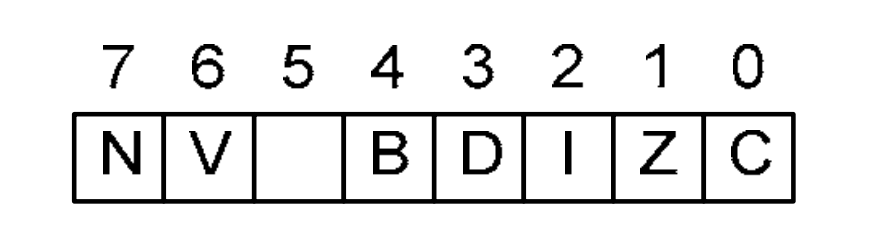
\includegraphics[width=0.5\textwidth]{status.png}}
\end{figure}
\end{itemize}

\section {Interrupciones}
Las interrupciones pueden ser generadas por software y por hardware. La NES tiene tres tipos diferentes que son NMI, IRQ y reset. Las direcciones a la cual saltar cuando una interrupción ocurre son guardadas en un arreglo (o vector table) en el PRG-ROM en \$FFFA-\$FFFF. Cuando una interrupción ocurre el sistema performa las siguientes acciones:
\begin{enumerate}
\item Reconocer el pedido de interrupción que ocurrió.
\item Completar la ejecución de la instrucción actual.
\item Poner el program counter y el status register en el stack
\item Activar el flag interrupt disable para prevenir interrupciones más adelante.
\item Cargar la dirección de la rutina encargada de procesar la interrupción desde la vector table al program counter.
\item Ejecutar la rutina correspondiente.
\item Luego de ejecutar la instrucción RTI (Return From Interrupt), obtener el program counter y el status desde el stack.
\item Continuar la ejecución del programa.
\end{enumerate}

Las \textbf{IRQs}, también llamadas maskable interrupt, son generadas por algunos memory mappers. Pueden ser iniciadas por software usando la instruccion BRK (Break). Cuando una IRQ ocurre el sistema salta a la dirección \$FFFE-\$FFFF.

La \textbf{NMI} (Non-Maskable Interrupt) es una interrupción generada por la PPU cuando la V-Blank ocurre al final de cada frame. NMI no es afectadas por el bit de interrupt disable. Sin embargo, NMI puede ser desactivada si el bit 7 del registro de control 1 del PPU (\$2000) es limpiado. Cuando una NMI ocurre el sistema salta a la dirección localizada en \$FFFA-\$FFFB.

La interrupción reset es iniciada al comienzo del sistema y cuando el usuario presiona el botón de reinicio. Cuando esta ocurre el sistema salta a la dirección \$FFFC-\$FFFD.

El sistema da mayor prioridad a las interrupción reset, seguida de NMI y finalmente IRQ.
La consola tiene una latencia de interrupción de 7 ciclos, que implica que tarda 7 ciclos del CPU para comenzar a ejecutar la rutina de interrupción.


\section{Modos de Acceso}
El 6502 tiene distintos modos de acceso, los cuales proveen distintas formas de acceder a memoria. Hay algunos que operan sobre los contenidos de registros. En total existen 13 modos distintos.

\section{Instrucciones}

El procesador tiene 56 instrucciones diferentes aunque algunas se repiten, usando distintos modos de acceso haciendo un total de 151 opcodes válidos de un posible total de 256. Las instrucciones tienen uno, dos o tres bytes de longitud, dependiendo del modo de acceso. El primer byte es el opcode y los restantes los operandos.

\subsection{Implementación}

Para sintetizar todas las instrucciones necesarias en el código, se descompuso cada instrucción en micro-operaciones. Por ejemplo para hacer un ADD (suma), primero se traen los operandos de memoria o de registros, luego se efectua la suma, después se guarda el resultado en el registro correspondiente y por último se modifican las flags del status register adecuadas. Cada uno de estos pasos es una micro-operación.

Si pudieramos aprovechar que que sólo se necesitan 56 micro-operaciones para poder expresar \emph{todas} las instrucciones del procesador, se podría simplificar mucho el diseño.


\begin{thebibliography}{9}

\bibitem{}
  OS Dev Wiki,
  
  disponible en \url{http://wiki.osdev.org/Main_Page}.
 
\bibitem{}
  Operating System Development Series,
  BrokenThorn Entertainment,
  
  disponible en \url{http://www.brokenthorn.com/Resources/OSDevIndex.html}.

\bibitem{}
  MosquitOS,
  Open-sourced hobby operating system,
  Tristan Seifert,
  
  disponible en \url{https://github.com/tristanseifert/MosquitOS}.
  
\bibitem{}
  Skelix OS Tutorials,
  Mo Xiaoming,
  
  disponible en \url{http://skelix.net/skelixos/index_en.html}.
 
\bibitem{}
  Cedille,
  A microkernel with a purpose - to keep most of the code out of the kernel,
  Corwin Mcknight,
  
  disponible en \url{https://github.com/Lionel07/Cedille}.
  
\bibitem{}
  pcore,
  Student project of OS kernel in C/C++,
  Korepwx,
  
  disponible en \url{https://github.com/korepwx/pcore}.

\bibitem{}
  A small hobby OS,
  Eduardo Veiga,
  
  disponible en \url{https://github.com/cinemascop89/kernel}.


\bibitem{}
  Creating a NES emulator in C++11,
  Joel Yliluoma (Bisqwit),
  disponible en \url{https://www.youtube.com/watch?v=y71lli8MS8s}.

\bibitem{nesdoc}
  Nintendo Entertainment System Documentation,
  Patrick Diskin,
  
  disponible en \url{http://nesdev.com/NESDoc.pdf}.
  
\bibitem{}
  NES Devolpment Wiki,
  
  disponible en \url{http://wiki.nesdev.com/w/index.php/Nesdev}.
  
\bibitem{techdocs}
  NES Technical Documents,
  
  disponible en \url{http://www.castledragmire.com/hynes/reference/docs/}.



\end{thebibliography}

%-----------------------------------------------------------
\end{document}
